\documentclass[10pt,letterpaper]{hmcpset}
\usepackage[margin=1in]{geometry}
\usepackage{graphicx}
\usepackage{amsmath,amssymb}
\usepackage[T1]{fontenc}

\newcommand{\aln}[1]{\begin{align*} #1 \end{align*}} %fast align

\assignment{Hillar, Windfeldt Section 1 Problems}
\name{Max Comstock}
\class{Professor Omar}
\duedate{Summer 2014}

\begin{document}

\begin{problem}[1]
Let $G$ be the following 3-coloring of the following graph:
\begin{center}
	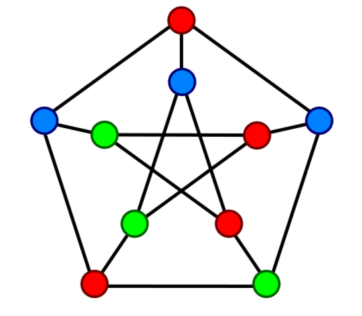
\includegraphics[width=2in]{3coloring.png}
\end{center}
Using Definition 1.4, write down a $\nu$-basis for $G$, and hence find a generating set for $A_\nu$. (Label the vertices with the labels $1,2,\ldots,10$ in any way you like.)
\end{problem}

\begin{solution}
The $\nu$-basis is
\aln{
	g_1 &= x_1 - x_8\\
	g_2 &= x_2 - x_6\\
	g_3 &= x_3 - x_{10}\\
	g_4 &= x_4 - x_8\\
	g_5 &= x_5 - x_6\\
	g_6 &= x_6 + x_8 + x_{10}\\
	g_7 &= x_7 - x_8\\
	g_8 &= x_8^2 + x_8 x_{10} + x_{10}^2\\
	g_9 &= x_9 - x_{10}\\
	g_{10} &= x_{10}^3 - 1
}
\end{solution}


\begin{problem}[2]
Read example 1.8 and verify the computations in this example using Macaulay 2.
\end{problem}

\begin{solution}
This has been verified using Macaulay 2.
\end{solution}

\newpage

\begin{problem}[3]
Using the definition before Theorem 1.11, write down the reduced $\nu$-basis for the ideal $A_\nu$ from Problem 1 in this problem set. Use Macaulay 2 to verify that $G$ from Problem 1 violates the conclusion in Theorem 1.11.
\end{problem}

\begin{solution}
The reduced $\nu$-basis is
\aln{
	\tilde{g}_1 &= x_1 - x_8\\
	\tilde{g}_2 &= x_2 + x_8 + x_{10}\\
	\tilde{g}_3 &= x_3 - x_{10}\\
	\tilde{g}_4 &= x_4 - x_8\\
	\tilde{g}_5 &= x_5 + x_8 + x_{10}\\
	\tilde{g}_6 &= x_6 + x_8 + x_{10}\\
	\tilde{g}_7 &= x_7 - x_8\\
	\tilde{g}_8 &= x_8^2 + x_8 x_{10} + x_{10}^2\\
	\tilde{g}_9 &= x_9 - x_{10}\\
	\tilde{g}_{10} &= x_{10}^3 - 1
}
\end{solution}


\begin{problem}[4]
Use Macaulay 2 to verify Example 1.13.
\end{problem}

\begin{solution}
This has been verified using Macaulay 2.
\end{solution}



\end{document}
